%-----------------------Homework------------------------------------
%-------------------Arman Shokrollahi---------------------------------
%---------------------Coding Theory-------------------------------

\documentclass[a4 paper]{article}
% Set target color model to RGB
\usepackage[inner=1.5cm,outer=1.5cm,top=2.5cm,bottom=2.5cm]{geometry}
\usepackage{setspace}
\usepackage[rgb]{xcolor}
\usepackage{pythonhighlight}
\usepackage{caption}
\usepackage{subcaption}
\usepackage{pdfpages}
\usepackage{verbatim}
\usepackage{amsgen,amsmath,amstext,amsbsy,amsopn,tikz,amssymb,tkz-linknodes}
\usepackage{fancyhdr}
\usepackage[colorlinks=true, urlcolor=blue,  linkcolor=blue, citecolor=blue]{hyperref}
\usepackage[colorinlistoftodos]{todonotes}
\usepackage{rotating}
%\usetikzlibrary{through,backgrounds}
\hypersetup{%
pdfauthor={Arman Shokrollahi},%
pdftitle={Homework},%
pdfkeywords={Tikz,latex,bootstrap,uncertaintes},%
pdfcreator={PDFLaTeX},%
pdfproducer={PDFLaTeX},%
}
%\usetikzlibrary{shadows}
\usepackage[francais]{babel}
\usepackage{booktabs}
\newcommand{\ra}[1]{\renewcommand{\arraystretch}{#1}}

      \newtheorem{thm}{Theorem}[section]
      \newtheorem{prop}[thm]{Proposition}
      \newtheorem{lem}[thm]{Lemma}
      \newtheorem{cor}[thm]{Corollary}
      \newtheorem{defn}[thm]{Definition}
      \newtheorem{rem}[thm]{Remark}
      \numberwithin{equation}{section}

\newcommand{\homework}[6]{
   \pagestyle{myheadings}
   \thispagestyle{plain}
   \newpage
   \setcounter{page}{1}
   \noindent
   \begin{center}
   \framebox{
      \vbox{\vspace{2mm}
    \hbox to 6.28in { {\bf JWST Project \hfill} }
       \vspace{6mm}
       \hbox to 6.28in { {\Large \hfill #1 (#2)  \hfill} }
       \vspace{6mm}
       \hbox to 6.28in { {\it Instructor: #3 \hfill Student: #5} }
       %\hbox to 6.28in { {\it TA: #4  \hfill #6}}
      \vspace{2mm}}
   }
   \end{center}
   \markboth{#5 -- #1}{#5 -- #1}
   \vspace*{4mm}
}

\newcommand{\bbF}{\mathbb{F}}
\newcommand{\bbX}{\mathbb{X}}
\newcommand{\bI}{\mathbf{I}}
\newcommand{\bX}{\mathbf{X}}
\newcommand{\bY}{\mathbf{Y}}
\newcommand{\bepsilon}{\boldsymbol{\epsilon}}
\newcommand{\balpha}{\boldsymbol{\alpha}}
\newcommand{\bbeta}{\boldsymbol{\beta}}
\newcommand{\0}{\mathbf{0}}

\begin{document}
\homework{Meeting Notes \#12}{due \today}{McCleary}{}{Eddie Berman}{}
{\begin{tikzpicture}[outline/.style={draw=#1,thick,fill=#1!50}]
\node [outline=red] at (0,1) {\bf Agenda};
\end{tikzpicture}}
\begin{enumerate}
    \item Show current Plots \& progress
\end{enumerate}

\begin{figure}[!htb]
    \centering
    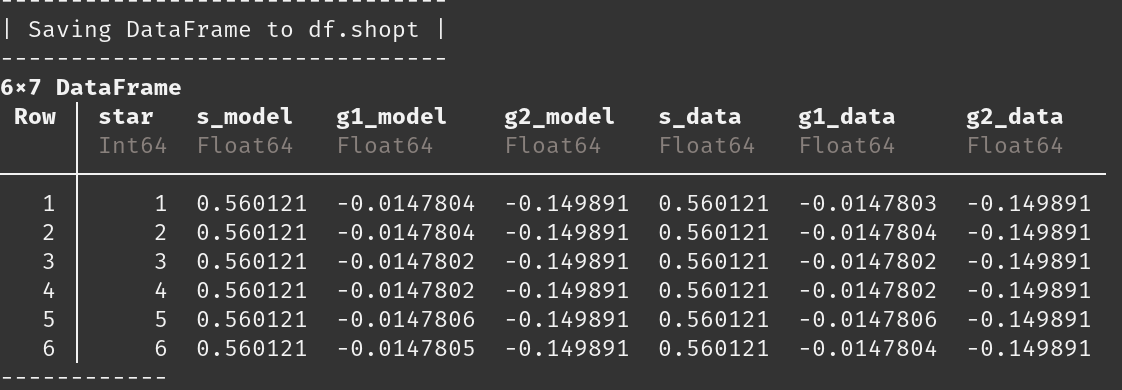
\includegraphics[scale=0.333]{Screenshot from 2023-05-15 13-11-48.png}
    \caption{df.shopt}
    \label{fig:my_label}
\end{figure}
\begin{figure}[!htb]
    \centering
    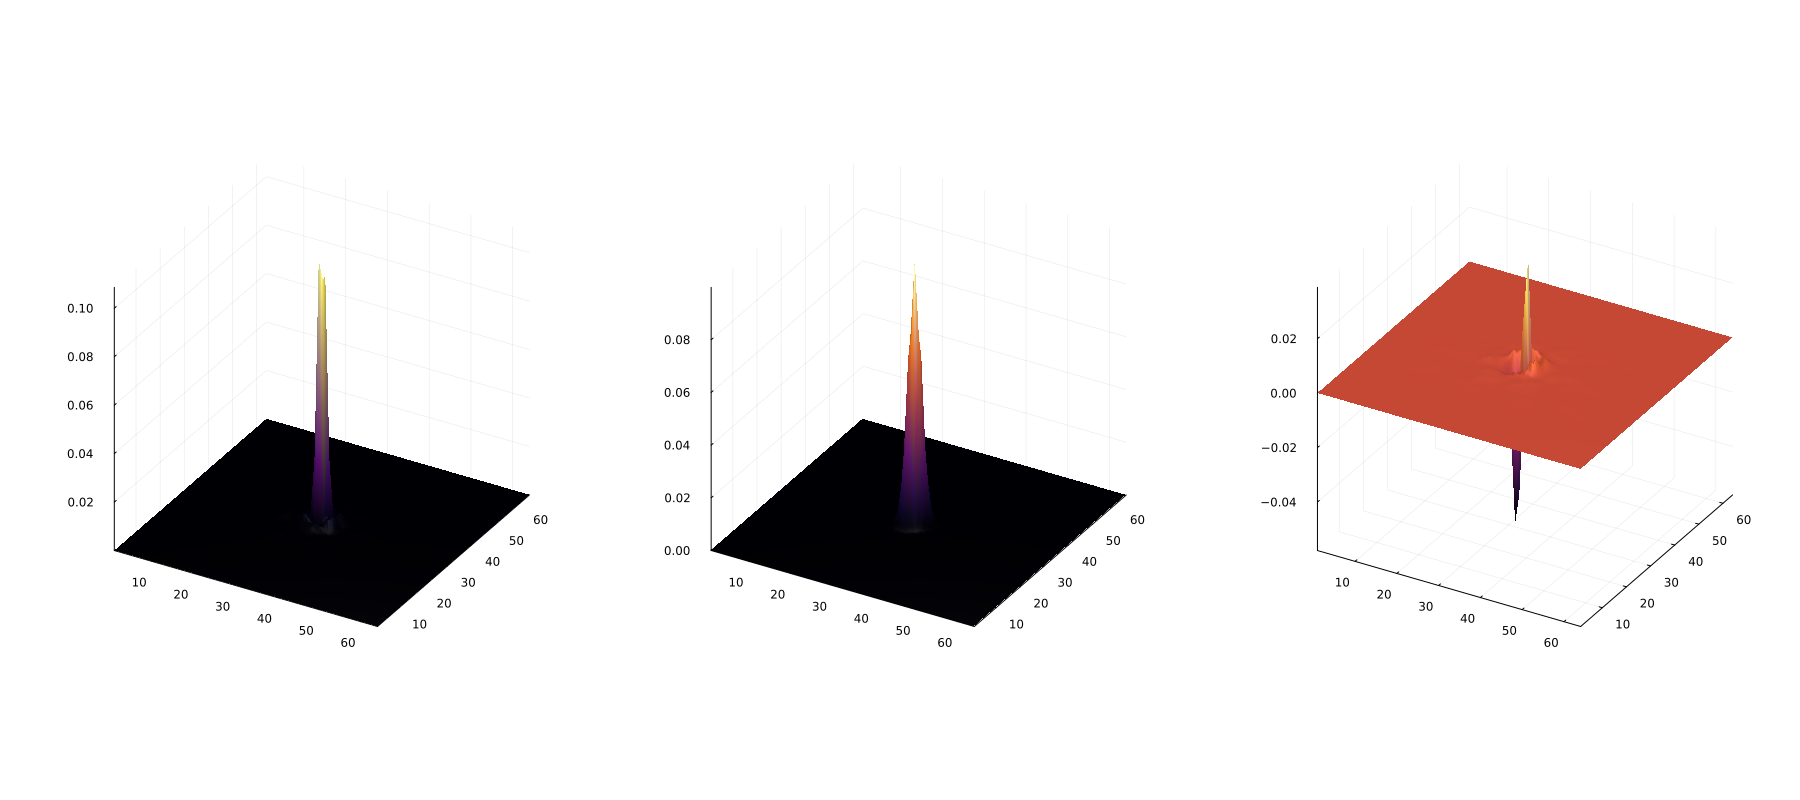
\includegraphics[scale=0.25]{3dAnalyticFit.png}
    \caption{3d analytic fit}
    \label{fig:my_label}
\end{figure}
\begin{figure}[!htb]
    \centering
    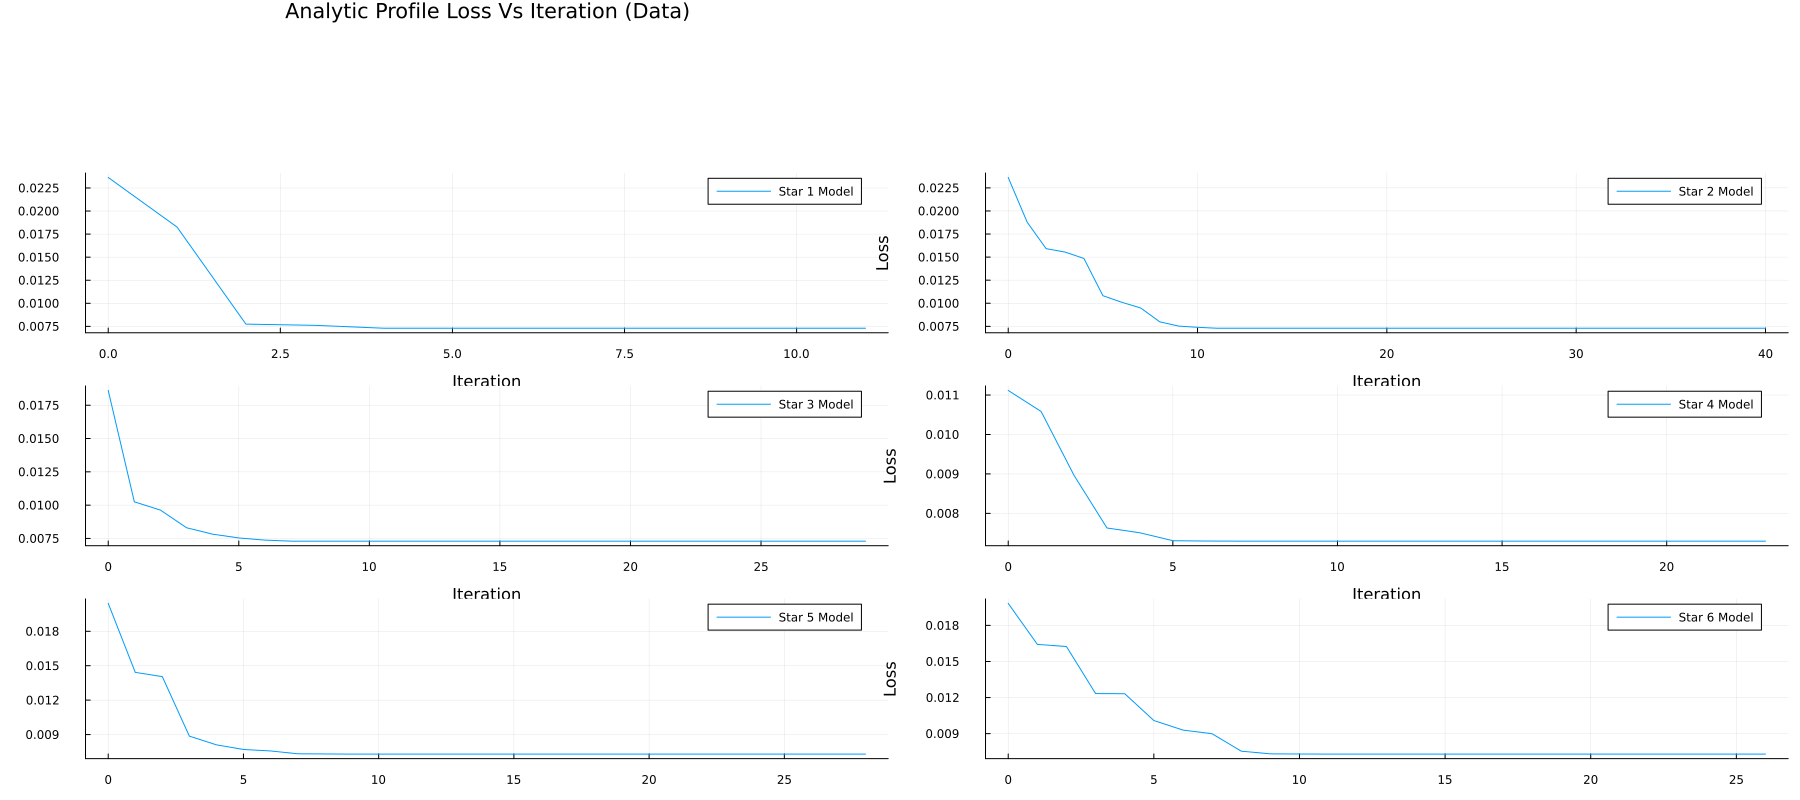
\includegraphics[scale=0.25]{lossTimeData.png}
    \caption{Loss Time Data}
    \label{fig:my_label}
\end{figure}
\begin{figure}[!htb]
    \centering
    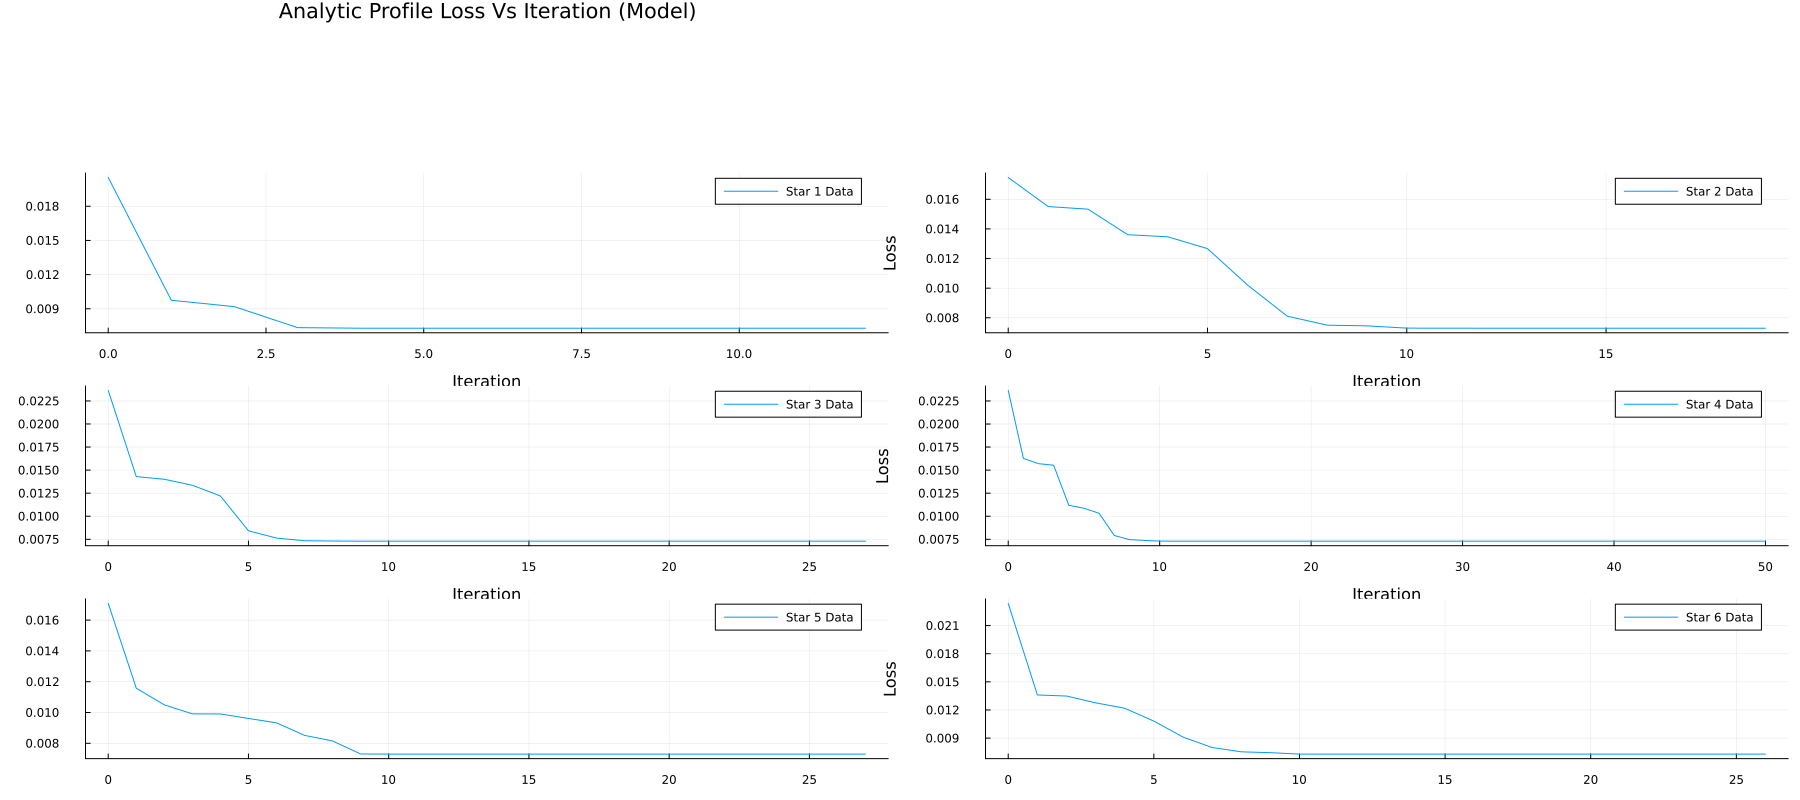
\includegraphics[scale=0.25]{lossTimeModel.png}
    \caption{Loss Time Model}
    \label{fig:my_label}
\end{figure} 
\begin{figure}[!htb]
    \centering
    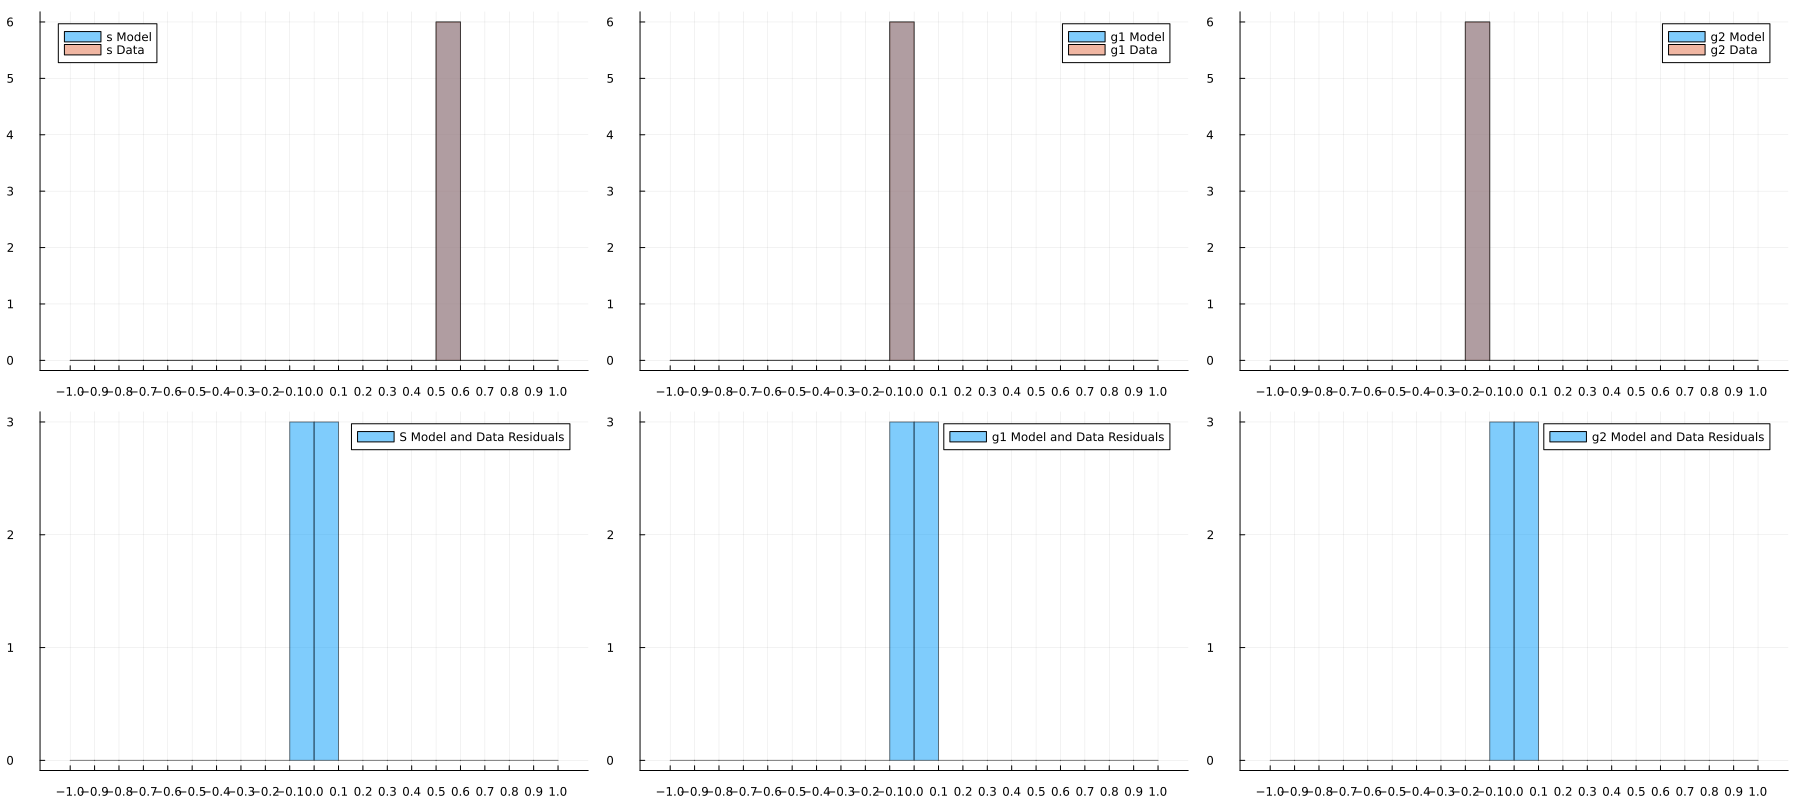
\includegraphics[scale=0.25]{parametersHistogram.png}
    \caption{Histogram}
    \label{fig:my_label}
\end{figure}
\begin{figure}[!htb]
    \centering
    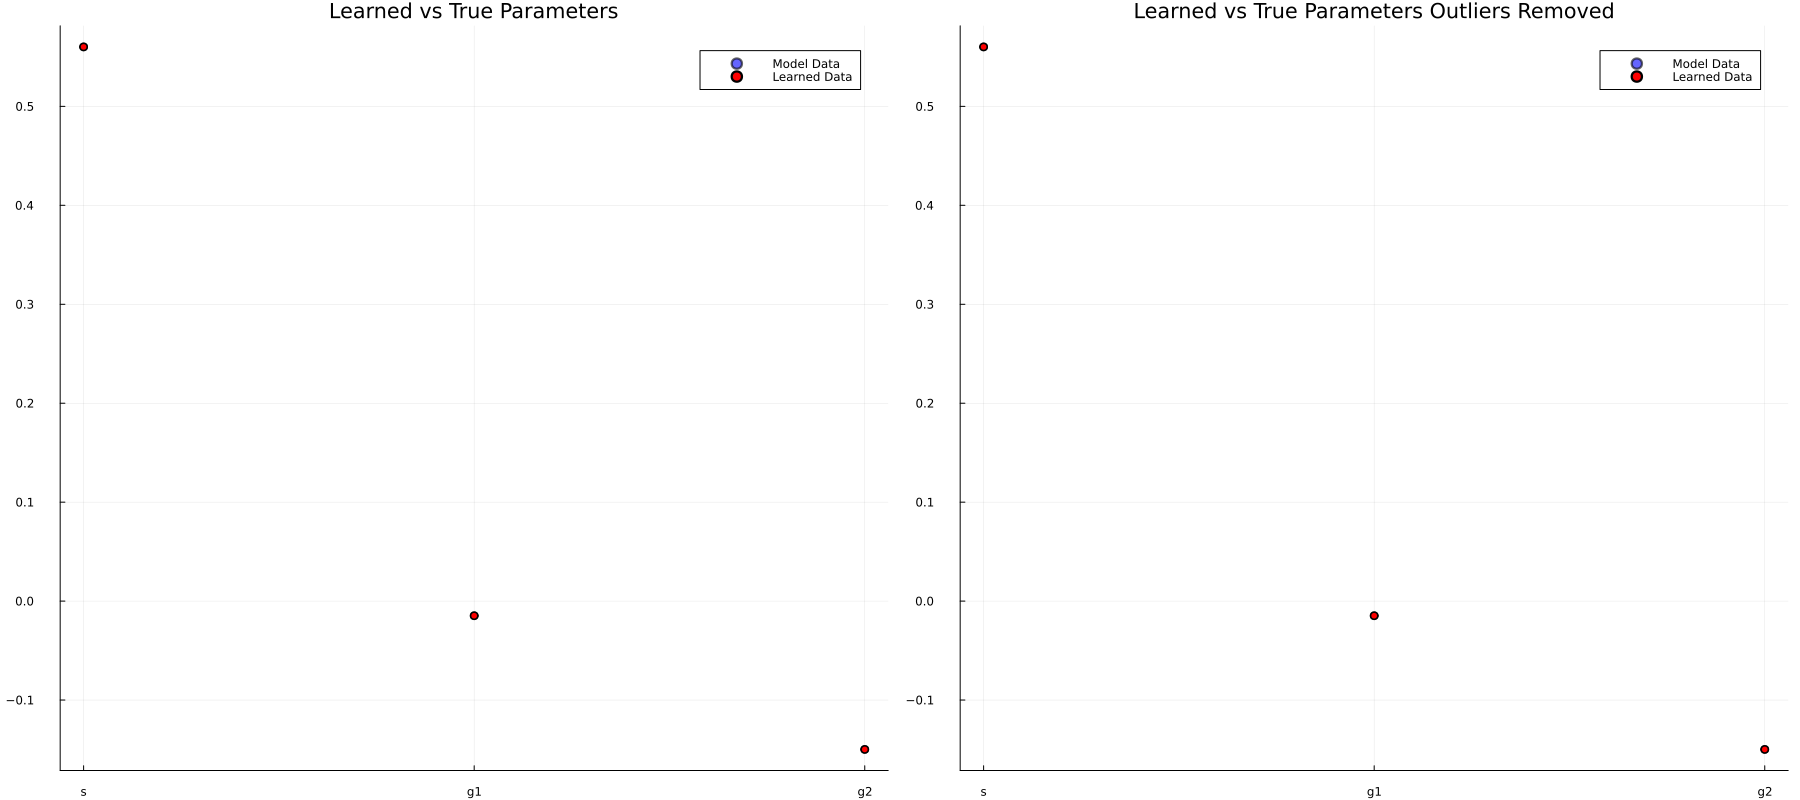
\includegraphics[scale=0.25]{parametersScatterplot.png}
    \caption{Scatterplot}
    \label{fig:my_label}
\end{figure}
\begin{figure}[!htb]
    \centering
    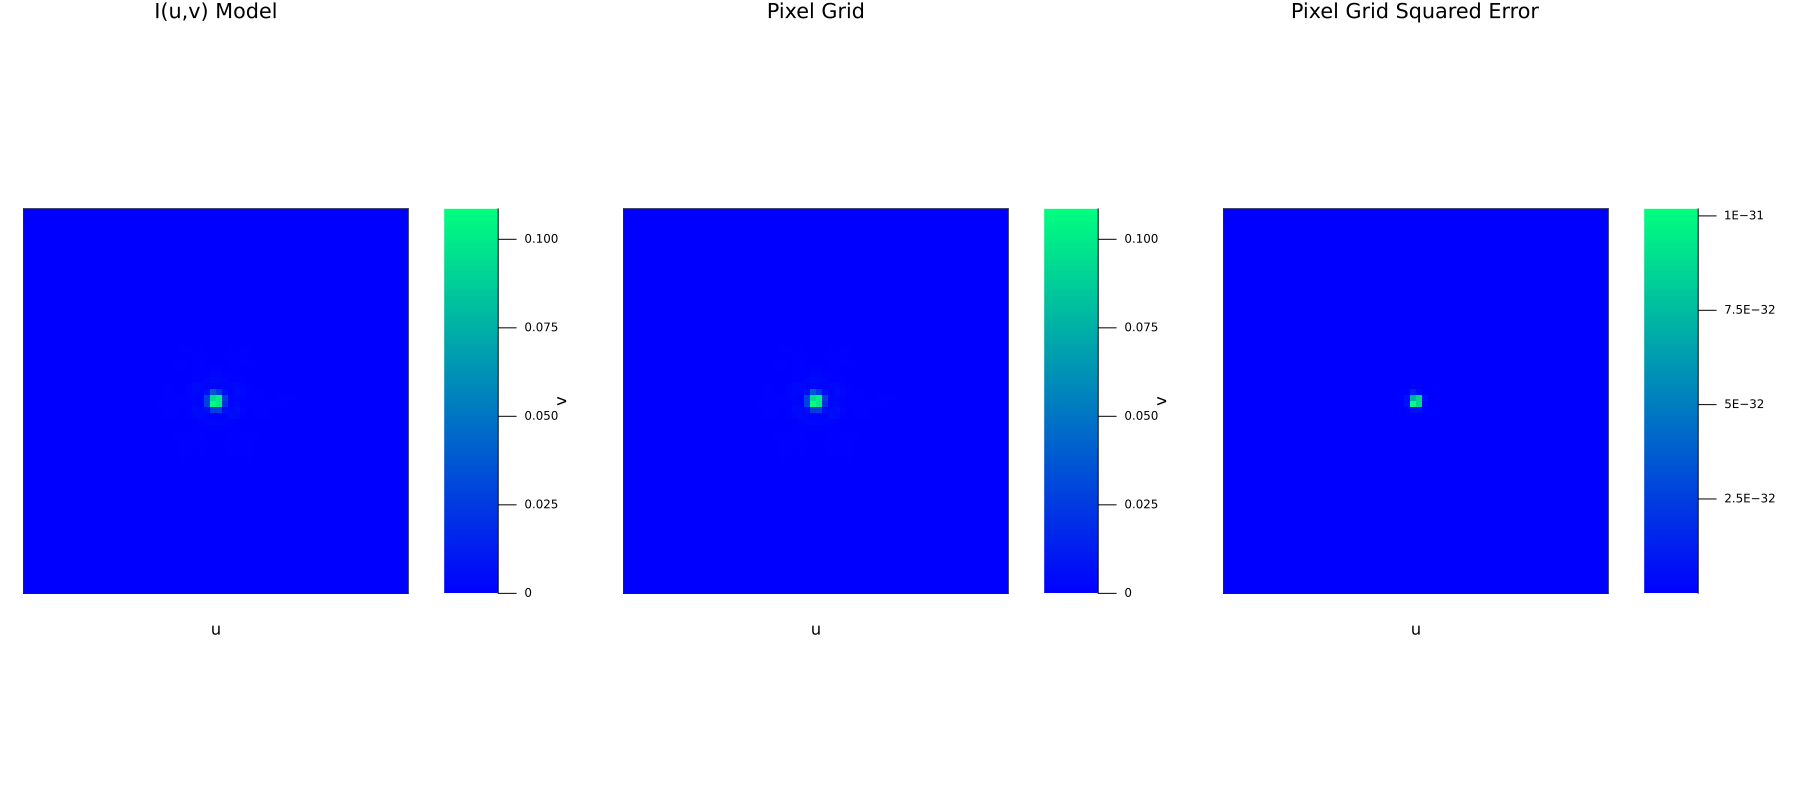
\includegraphics[scale=0.25]{pixelGridFit.png}
    \caption{Pixel Grid Fit}
    \label{fig:my_label}
\end{figure}
\begin{figure}[!htb]
    \centering
    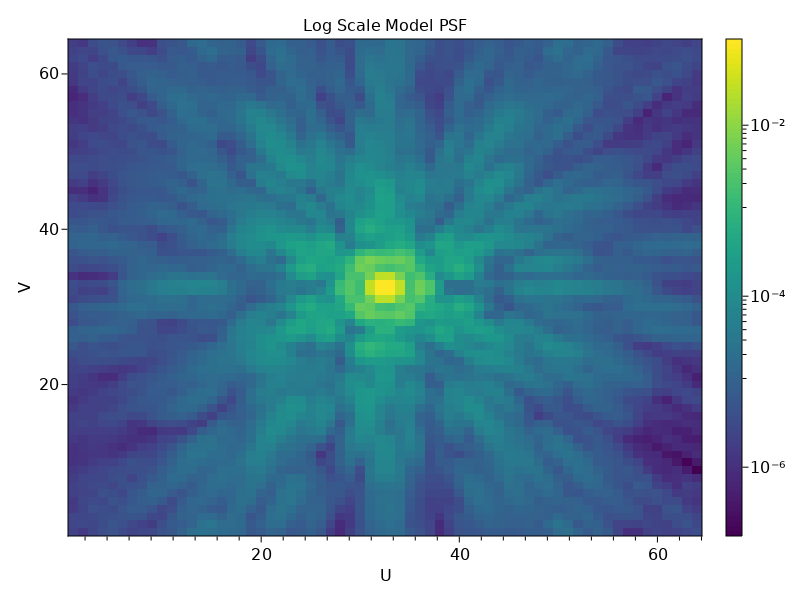
\includegraphics[scale=0.25]{test.png}
    \caption{log scale attempt}
    \label{fig:my_label}
\end{figure}

\clearpage
\noindent {\fbox{\it To-Do}}\\
\begin{enumerate}
    \item $\rho$ statistics
    \item plot fiexs (# stars)
    \item $(x,y) \rightarrow (u,v) , \left[ uv-map? \right]$
    \item kaisser squares
    \item Chi-Square fix
    \item catalog reading (borrow python code?)
    \item misc code cleanup
\end{enumerate}

\end{document}